\section{Durchführung}
\label{sec:Durchführung}
\subsection{Versuchsaufbau}
Für diesen Versuch wird ein Aufbau verwendet, wie in \autoref{fig:Aufbau} zu sehen ist. Unter die transparente Glasplatte
lassen sich verschiedene Winkelskalen legen, über die Einfalls- und Ausfallswinkel bestimmt werden können.
\begin{figure}[H]
    \centering
    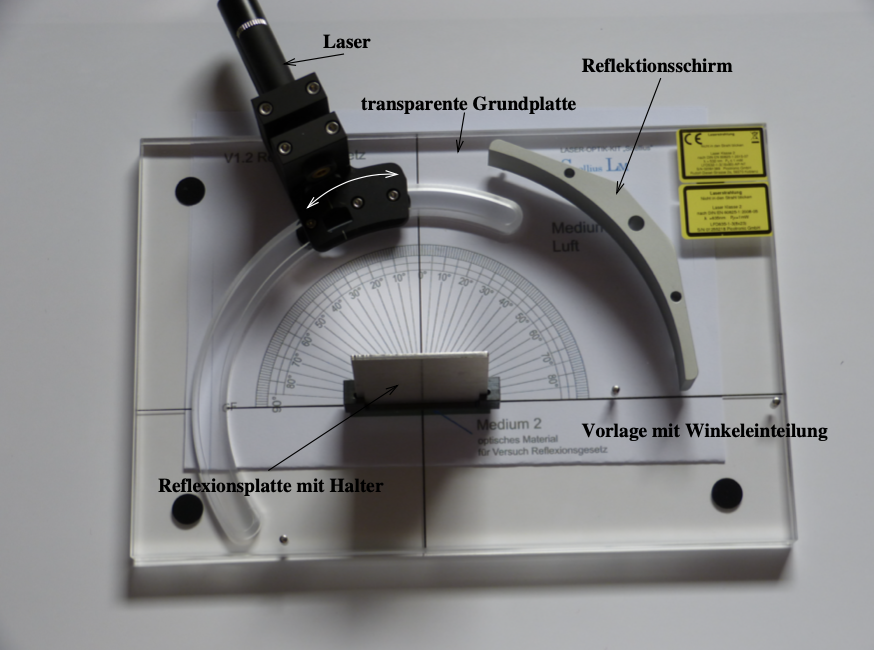
\includegraphics[height=7.5cm]{content/pics/Aufbau_1.png}
    \caption{Aufbau des Versuchs mit Beschriftungen der einzelnen Bauteile \cite{v400}.}
    \label{fig:Aufbau}
\end{figure}
Anstelle der eingezeichneten Relexionsplatte lassen sich auch andere optische Elemente, wie ein Prisma oder eine
planparallele Platte, in den Aufbau integrieren.
Als Lichtquelle werden ein grüner und ein roter Laser mit den Wellenlängen von 
$\lambda_{\text{grün}} = \qty{532}{\nano\metre}$ und $\lambda_{\text{rot}} = \qty{635}{\nano\metre}$ verwendet.

\subsection{Reflexionsgesetz}
Zur Überprüfung des Reflexionsgesetzes wird in der Halterung ein Spiegel installiert und wird unter 7 verschiedenen
Winkeln mit grünem Laserlicht bestrahlt. Mithilfe einer passenden Winkelskala unter dem Versuchsaufbau werden Einfalls-
und Ausfallswinkel bestimmt.

\subsection{Brechungsgesetz}
Anstelle des Spiegels wird eine planparallele Platte in den Aufbau eingesetzt. In diese wird erneut unter 7 verschiedenen
Einfallswinkeln grünes Laserlicht eingestrahlt. An einer Kante der planparallelen Platte lässt sich über eine Winkelskala
der Brechungswinkel abgelesen.

\subsection{Prisma}
In einem nächsten Schritt wird ein Prisma in den Versuchsaufbau integriert. Außerdem wird an der unteren Kante eine 
horizontale Winkelskala platziert, mithilfe derer die Austrittswinkel für rotes und grünes Laserlicht gemessen werden.
Hierbei werden gleiche 5 Eintrittswinkel für beide Laserstrahlen im Bereich von $\qty{10}{\degree} ≤ \alpha_1 ≤ \qty{60}{\degree}$
gewählt.

\subsection{Gitter}
Das Prisma wird nun durch ein Gitter ersetzt und es werden die sichtbaren Intesitätsmaxima für grünes und rotes Laserlicht
abgelesen. Dafür wird eine andere Winkelskala als Schirm verwendet. Dieser Teil des Versuches wird für Gitter mit 100, 300, und
600 Linien pro Millimeter durchgeführt.

\subsection{Vorbereitungsaufgaben}
In Vorbereitung auf die tatsächliche Durchführung des Versuchs sind einige Brechungsindices herauszusuchen, die in 
\autoref{tab:Brechungsindices} dargestellt sind.
\begin{table}[H]
    \centering
    \caption{Brechungsindices verschiedener Materialien.}
    \label{tab:Brechungsindices}
    \begin{tabular}{S S S}
        \toprule
        {Material} & {Brechungsindex $n$} \\
        \midrule
        {Luft}      & {$\num{1,0003}$\,\cite{Brechungsindex_Wien}} \\ 
        {Wasser}    & {$\num{1,333}$\,\cite{Brechungsindex_Wien}} \\  
        {Kronglas}  & {$\num{1,510}$\,\cite{Brechungsindex}} \\ 
        {Plexiglas} & {$\num{1,490}$\,\cite{Brechungsindex}} \\ 
        {Diamant}   & {$\num{2,417}$\,\cite{Brechungsindex_Wien}} \\ 
        \bottomrule
    \end{tabular}
  \end{table}
  Außerdem wird die Gitterkostante für Gitter mit 600, 300, und 100 Linien pro Millimeter bestimmt.
  \begin{table}[H]
    \centering
    \caption{Gitterkonstanten für Gitter mit 600, 300, und 100 Linien pro Millimeter.}
    \label{tab:Gitter}
    \begin{tabular}{S S}
        \toprule
        {Linien\,/\,mm} & {$d \mathbin{/} \unit{\micro\metre}$} \\
        \midrule
        $\num{600}$ & $\frac{10}{6}$ \\
        $\num{300}$ & $\frac{10}{3}$ \\
        $\num{100}$ & $\num{10}$     \\ 
        \bottomrule
    \end{tabular}
  \end{table}